\documentclass{standalone}
\usepackage{tikz}
\usetikzlibrary{patterns, positioning}


\begin{document}
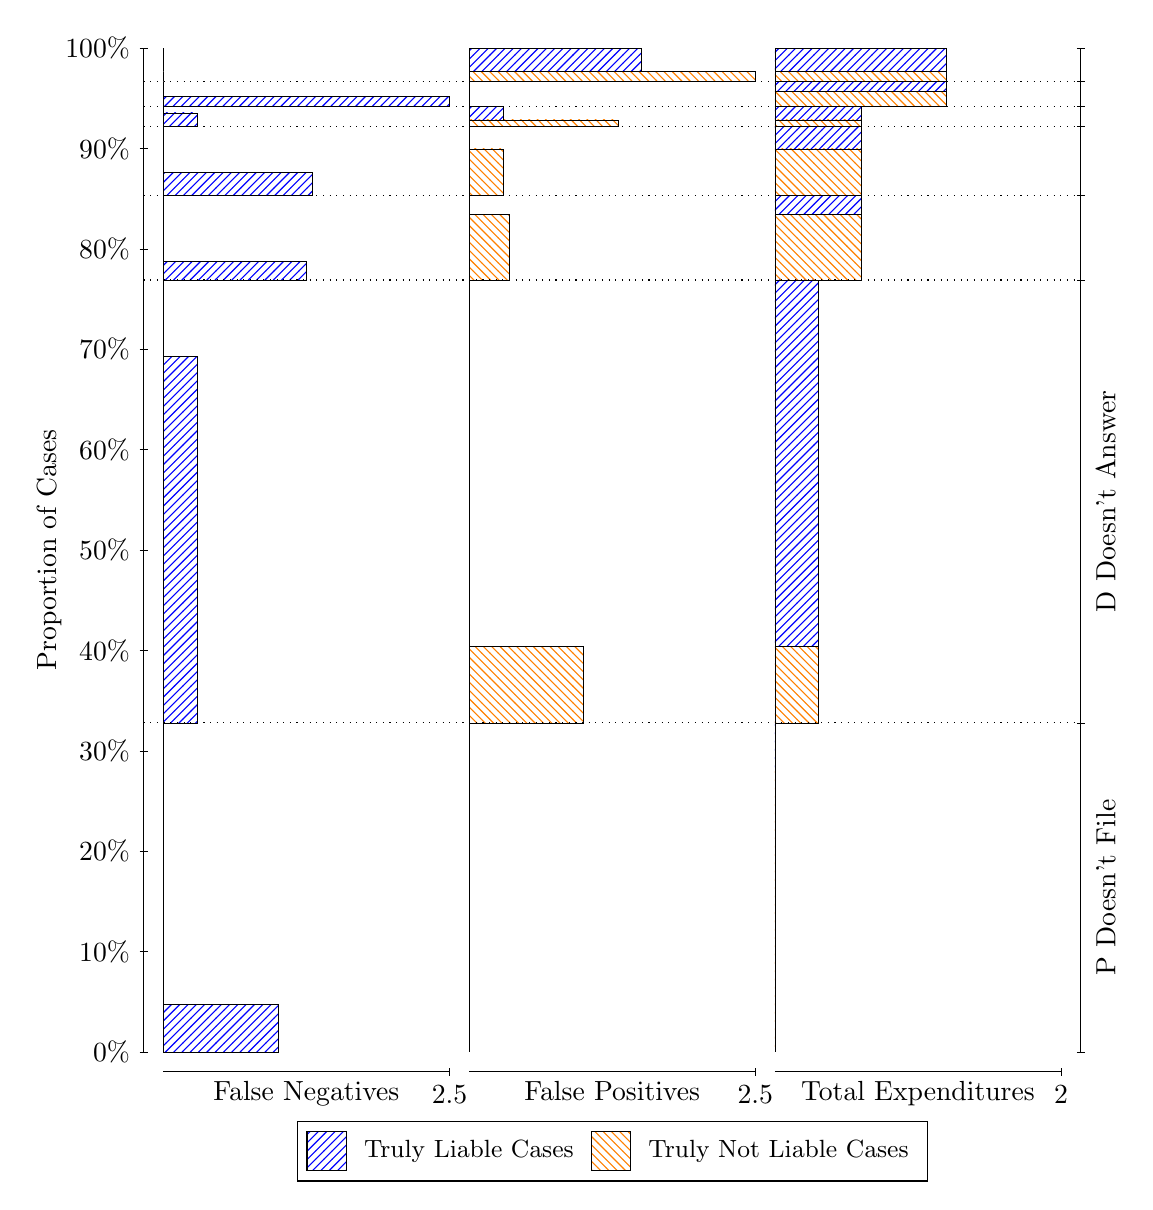
\begin{tikzpicture}
\draw[black, very thin] (1.5,1.75) -- (1.5,14.5);
\node[rotate=90, text=black, anchor=center] at (0.3, 8.125) {Proportion of Cases};
\draw[black, very thin] (1.45,1.75) -- (1.55,1.75);
\node[text=black, anchor=east] at (1.45, 1.75) {0\%};
\draw[black, very thin] (1.45,3.025) -- (1.55,3.025);
\node[text=black, anchor=east] at (1.45, 3.025) {10\%};
\draw[black, very thin] (1.45,4.3) -- (1.55,4.3);
\node[text=black, anchor=east] at (1.45, 4.3) {20\%};
\draw[black, very thin] (1.45,5.575) -- (1.55,5.575);
\node[text=black, anchor=east] at (1.45, 5.575) {30\%};
\draw[black, very thin] (1.45,6.85) -- (1.55,6.85);
\node[text=black, anchor=east] at (1.45, 6.85) {40\%};
\draw[black, very thin] (1.45,8.125) -- (1.55,8.125);
\node[text=black, anchor=east] at (1.45, 8.125) {50\%};
\draw[black, very thin] (1.45,9.4) -- (1.55,9.4);
\node[text=black, anchor=east] at (1.45, 9.4) {60\%};
\draw[black, very thin] (1.45,10.675) -- (1.55,10.675);
\node[text=black, anchor=east] at (1.45, 10.675) {70\%};
\draw[black, very thin] (1.45,11.95) -- (1.55,11.95);
\node[text=black, anchor=east] at (1.45, 11.95) {80\%};
\draw[black, very thin] (1.45,13.225) -- (1.55,13.225);
\node[text=black, anchor=east] at (1.45, 13.225) {90\%};
\draw[black, very thin] (1.45,14.5) -- (1.55,14.5);
\node[text=black, anchor=east] at (1.45, 14.5) {100\%};

\draw[black, very thin] (13.4,1.75) -- (13.4,14.5);
\draw[black, very thin] (13.35,1.75) -- (13.45,1.75);
\node[anchor=west] at (13.35, 1.75) {};
\draw[black, very thin] (13.35,5.9302) -- (13.45,5.9302);
\node[anchor=west] at (13.35, 5.9302) {};
\draw[black, very thin] (13.35,11.554) -- (13.45,11.554);
\node[anchor=west] at (13.35, 11.554) {};
\draw[black, very thin] (13.35,12.631) -- (13.45,12.631);
\node[anchor=west] at (13.35, 12.631) {};
\draw[black, very thin] (13.35,13.507) -- (13.45,13.507);
\node[anchor=west] at (13.35, 13.507) {};
\draw[black, very thin] (13.35,13.758) -- (13.45,13.758);
\node[anchor=west] at (13.35, 13.758) {};
\draw[black, very thin] (13.35,14.078) -- (13.45,14.078);
\node[anchor=west] at (13.35, 14.078) {};
\draw[black, very thin] (13.35,14.5) -- (13.45,14.5);
\node[anchor=west] at (13.35, 14.5) {};

\draw[black, very thin, pattern color=blue, pattern=north east lines] (1.75,1.75) rectangle (3.2033,2.3513);
\draw[black, very thin, pattern color=orange, pattern=north west lines] (1.75,2.3513) rectangle (1.75,5.9302);
\draw[black, very thin, pattern color=blue, pattern=north east lines] (1.75,5.9302) rectangle (2.186,10.585);
\draw[black, very thin, pattern color=orange, pattern=north west lines] (1.75,10.585) rectangle (1.75,11.554);
\draw[black, very thin, pattern color=blue, pattern=north east lines] (1.75,11.554) rectangle (3.5667,11.793);
\draw[black, very thin, pattern color=orange, pattern=north west lines] (1.75,11.793) rectangle (1.75,12.631);
\draw[black, very thin, pattern color=blue, pattern=north east lines] (1.75,12.631) rectangle (3.6393,12.917);
\draw[black, very thin, pattern color=orange, pattern=north west lines] (1.75,12.917) rectangle (1.75,13.507);
\draw[black, very thin, pattern color=blue, pattern=north east lines] (1.75,13.507) rectangle (2.186,13.677);
\draw[black, very thin, pattern color=orange, pattern=north west lines] (1.75,13.677) rectangle (1.75,13.758);
\draw[black, very thin, pattern color=blue, pattern=north east lines] (1.75,13.758) rectangle (5.3833,13.884);
\draw[black, very thin, pattern color=orange, pattern=north west lines] (1.75,13.884) rectangle (1.75,14.078);
\draw[black, very thin, pattern color=orange, pattern=north west lines] (1.75,14.078) rectangle (1.75,14.204);
\draw[black, very thin, pattern color=blue, pattern=north east lines] (1.75,14.204) rectangle (1.75,14.5);
\draw[black, very thin, pattern color=orange, pattern=north west lines] (5.6333,1.75) rectangle (5.6333,5.3289);
\draw[black, very thin, pattern color=blue, pattern=north east lines] (5.6333,5.3289) rectangle (5.6333,5.9302);
\draw[black, very thin, pattern color=orange, pattern=north west lines] (5.6333,5.9302) rectangle (7.0867,6.899);
\draw[black, very thin, pattern color=blue, pattern=north east lines] (5.6333,6.899) rectangle (5.6333,11.554);
\draw[black, very thin, pattern color=orange, pattern=north west lines] (5.6333,11.554) rectangle (6.142,12.391);
\draw[black, very thin, pattern color=blue, pattern=north east lines] (5.6333,12.391) rectangle (5.6333,12.631);
\draw[black, very thin, pattern color=orange, pattern=north west lines] (5.6333,12.631) rectangle (6.0693,13.22);
\draw[black, very thin, pattern color=blue, pattern=north east lines] (5.6333,13.22) rectangle (5.6333,13.507);
\draw[black, very thin, pattern color=orange, pattern=north west lines] (5.6333,13.507) rectangle (7.5227,13.587);
\draw[black, very thin, pattern color=blue, pattern=north east lines] (5.6333,13.587) rectangle (6.0693,13.758);
\draw[black, very thin, pattern color=orange, pattern=north west lines] (5.6333,13.758) rectangle (5.6333,13.953);
\draw[black, very thin, pattern color=blue, pattern=north east lines] (5.6333,13.953) rectangle (5.6333,14.078);
\draw[black, very thin, pattern color=orange, pattern=north west lines] (5.6333,14.078) rectangle (9.2667,14.204);
\draw[black, very thin, pattern color=blue, pattern=north east lines] (5.6333,14.204) rectangle (7.8133,14.5);
\draw[black, very thin, pattern color=orange, pattern=north west lines] (9.5167,1.75) rectangle (9.5167,5.3289);
\draw[black, very thin, pattern color=blue, pattern=north east lines] (9.5167,5.3289) rectangle (9.5167,5.9302);
\draw[black, very thin, pattern color=orange, pattern=north west lines] (9.5167,5.9302) rectangle (10.062,6.899);
\draw[black, very thin, pattern color=blue, pattern=north east lines] (9.5167,6.899) rectangle (10.062,11.554);
\draw[black, very thin, pattern color=orange, pattern=north west lines] (9.5167,11.554) rectangle (10.607,12.391);
\draw[black, very thin, pattern color=blue, pattern=north east lines] (9.5167,12.391) rectangle (10.607,12.631);
\draw[black, very thin, pattern color=orange, pattern=north west lines] (9.5167,12.631) rectangle (10.607,13.22);
\draw[black, very thin, pattern color=blue, pattern=north east lines] (9.5167,13.22) rectangle (10.607,13.507);
\draw[black, very thin, pattern color=orange, pattern=north west lines] (9.5167,13.507) rectangle (10.607,13.587);
\draw[black, very thin, pattern color=blue, pattern=north east lines] (9.5167,13.587) rectangle (10.607,13.758);
\draw[black, very thin, pattern color=orange, pattern=north west lines] (9.5167,13.758) rectangle (11.697,13.953);
\draw[black, very thin, pattern color=blue, pattern=north east lines] (9.5167,13.953) rectangle (11.697,14.078);
\draw[black, very thin, pattern color=orange, pattern=north west lines] (9.5167,14.078) rectangle (11.697,14.204);
\draw[black, very thin, pattern color=blue, pattern=north east lines] (9.5167,14.204) rectangle (11.697,14.5);
\draw[black, dotted] (1.5,5.9302) -- (13.4,5.9302);
\draw[black, dotted] (1.5,11.554) -- (13.4,11.554);
\draw[black, dotted] (1.5,12.631) -- (13.4,12.631);
\draw[black, dotted] (1.5,13.507) -- (13.4,13.507);
\draw[black, dotted] (1.5,13.758) -- (13.4,13.758);
\draw[black, dotted] (1.5,14.078) -- (13.4,14.078);
\draw[black, very thin] (1.75,1.5) -- (5.3833,1.5);
\node[text=black, anchor=north] at (3.5667, 1.5) {False Negatives};
\draw[black, very thin] (5.3833,1.45) -- (5.3833,1.55);
\node[text=black, anchor=north] at (5.3833, 1.45) {2.5};

\draw[black, very thin] (5.6333,1.5) -- (9.2667,1.5);
\node[text=black, anchor=north] at (7.45, 1.5) {False Positives};
\draw[black, very thin] (9.2667,1.45) -- (9.2667,1.55);
\node[text=black, anchor=north] at (9.2667, 1.45) {2.5};

\draw[black, very thin] (9.5167,1.5) -- (13.15,1.5);
\node[text=black, anchor=north] at (11.333, 1.5) {Total Expenditures};
\draw[black, very thin] (13.15,1.45) -- (13.15,1.55);
\node[text=black, anchor=north] at (13.15, 1.45) {2};

\node[text=black, centered, rotate=90] at (13.72, 3.8401) {P Doesn't File};
\node[text=black, centered, rotate=90] at (13.72, 8.7422) {D Doesn't Answer};






\draw (7.449999999999999,1.5) node[draw=none] (baseCoordinate) {};
\begin{scope}[align=center]
        \matrix[scale=0.5, draw=black, below=0.5cm of baseCoordinate, nodes={draw}, column sep=0.1cm]{
            \node[rectangle, draw, minimum width=0.5cm, minimum height=0.5cm, pattern color=blue, pattern=north east lines] {}; &
            \node[draw=none, font=\small, text=black] (B) {Truly Liable Cases}; &
            \node[rectangle, draw, minimum width=0.5cm, minimum height=0.5cm, pattern color=orange, pattern=north west lines] {}; &
            \node[draw=none, font=\small, text=black] (B) {Truly Not Liable Cases}; \\
            };
\end{scope}

\end{tikzpicture}
\end{document}